\chapter{Graph Algorithms}

\section{Graph Theory Review}
Recall graph theory from MATH 239, specifically:
ms
\begin{defn}[graph]
  A graph $G$ is a pair $(V,E)$
  where $V$ is a finite set of \term{vertices}
  and $E$ is a set of unordered pairs of distinct vertices, called \term{edges}.
  By convention, we write $n = \abs{V}$ and $m = \abs{E}$.
\end{defn}

Now, we can define some structures on a graph:

\begin{defn}[adjacency list]
  An array $A[1..n]$ such that $A[v]$ is a linked list
  containing all edges connected to $v$.
  This contains $2m$ list cells with total size $\Theta(n+m)$
  but takes more than $O(1)$ time to test if an edge exists.
\end{defn}

\begin{defn}[adjacency matrix]
  A matrix $M \in M_{n\times n}(\{0,1\})$
  such that $M[v,w] = 1$ if and only if $\{v,w\} \in E$.
  Size is $\Theta(n^2)$ but testing if an edge exists is $O(1)$.
\end{defn}

\begin{example}
  Write the adjacency list and matrix for
  \tikz[baseline=-17pt]\graph{{1,5}--{2,4}--3[y=-0.5];1--5,2--4,2--5};
\end{example}
\begin{sol}
  The adjacency list is:
  \begin{enumerate}[1,nosep]
    \item $\to 2 \to 5$
    \item $\to 1 \to 3 \to 4 \to 5$
    \item $\to 2 \to 4$
    \item $\to 2 \to 3 \to 5$
    \item $\to 1 \to 2 \to 4$
  \end{enumerate}
  and the matrix is $M = \begin{bmatrix}
      0 & 1 & 0 & 0 & 1 \\
      1 & 0 & 1 & 1 & 1 \\
      0 & 1 & 0 & 1 & 0 \\
      0 & 1 & 1 & 0 & 1 \\
      1 & 1 & 0 & 1 & 0
    \end{bmatrix}$
\end{sol}

\begin{defn*}[graph terminology]
  We also recall some terms from MATH 239:
  \begin{itemize}[nosep]
    \item A \term{path} is a sequence of vertices $v_1,\dotsc,v_k$
          such that $\{v_i,v_{i+1}\} \in E$ for all $i$.
          If a path from $v$ to $w$ exists, we write $v \leadsto w$.
    \item A \term{connected graph} has $v \leadsto w$ for all $v,w \in V$.
    \item A \term{cycle} is a path $v \leadsto v$ of length at least 3
          with all elements pairwise distinct.
    \item A \term{tree} is a graph with no cycles.
    \item A \term{rooted tree} is a tree with a vertex chosen to be the \term{root}.
    \item A \term{subgraph} of $G = (V,E)$ is a graph $G' = (V',E')$
          where $V' \subseteq V$, $E' \subseteq E$, and $u,v \in V'$ for all $uv \in E'$.
    \item A \term{connected component} of $G$ is a connected subgraph of $G$
          that is not a subset of any other connected subgraph.
  \end{itemize}
\end{defn*}

\section{Breadth-First Search}

\begin{problem}
Search a graph $G$ starting from a vertex $s$
in order of distance from $s$.
\end{problem}

\begin{algorithm}
  \caption{\Call{BFS}{$G$, $s$}}
  \begin{algorithmic}[1]
    \State let $Q$ be an empty queue
    \State let $\vv{visited}$ be a boolean array of size $n$ with all entries set to $\bot$
    \State \Call{enqueue}{$s$, $Q$}
    \State $\vv{visited}[s] \gets \top$
    \While{$Q$ is not empty}
    \State $v \gets \Call{dequeue}{Q}$
    \For{$w$ neighbours of $v$} \label{line:bfs:forloop}
    \If{$\vv{visited}[w] = \bot$}
    \State \Call{enqueue}{$w$, $Q$}
    \State $\vv{visited}[w] \gets \top$
    \EndIf
    \EndFor
    \EndWhile
  \end{algorithmic}
\end{algorithm}

Each vertex is enqueued at most once and dequeued at most once,
which has cost $O(n)$.
Therefore, each adjacency list is read at most once.
The cost for the for loop is $O(\sum \deg v) = O(m)$ by the Handshaking Lemma.

Therefore, the total cost of \Call{BFS}{} is $O(n+m)$.

\begin{lemma}\label{lemma:bfs:visited}
  $\vv{visited}[v]$ is true for some vertex $v$
  if and only if $s \leadsto v$ in $G$.
\end{lemma}
\begin{prf}
  Let $s = v_0, \dotsc, v_K$ be the vertices with $\vv{visited}{v_i} = \top$,
  in order of discovery.
  By induction, we show that $s \leadsto v_i$.

  For $i = 0$, $v_0 = s$, so trivially $s \leadsto s$.

  Otherwise, suppose $s \leadsto v_j$ for all $j < i$.
  We are currently in the for loop for some vertex $w$ already visited.
  Therefore, by assumption, $s \leadsto w$.
  But since $v_i$ is a neighbour of $w$, $s \leadsto v_i$.
\end{prf}

\lecture{(05/30)}

\begin{xca}
  For a connected graph, $m \geq n - 1$.
\end{xca}
\begin{prf}
  Recall from MATH 239 that if a graph $G$ is connected, then it has a spanning tree $T$.
  The spanning tree of $n$ vertices has exactly $n-1$ edges.
  Then, since the spanning tree is a subgraph of $G$,
  $m \geq \abs{E(T)} = n-1$, as desired.
\end{prf}

\section{Shortest Path by BFS}

\begin{problem}
  What is the shortest path from $s$ to $v$ in $G$?
\end{problem}

Consider now how we can keep track of parents (predecessors)
and levels (depths):
\begin{algorithm}[H]
  \caption{\Call{BFS}{$G$, $s$} with parents and levels}
  \begin{algorithmic}[1]
    \State let $Q$ be an empty queue
    \State \textcolor{Green}{let $\vv{parent}$ be an array of size $n$ with all entries set to $\bot$}
    \State \textcolor{Green}{let $\vv{level}$ be an array of size $n$ with all entries set to $\infty$}
    \State \Call{enqueue}{$s$, $Q$}
    \State \textcolor{Green}{$\vv{parent}[s] \gets s$}
    \State \textcolor{Green}{$\vv{level}[s] \gets0$}
    \While{$Q$ is not empty}
    \State $v \gets \Call{dequeue}{Q}$
    \For{$w$ neighbours of $v$}
    \If{$\vv{parent}[w] = \bot$}
    \State \Call{enqueue}{$w$, $Q$}
    \State \textcolor{Green}{$\vv{parent}[w] \gets v$}
    \State \textcolor{Green}{$\vv{level}[w] \gets \vv{level}[v] + 1$}
    \EndIf
    \EndFor
    \EndWhile
  \end{algorithmic}
\end{algorithm}
We can define a \term{BFS tree} $T$ as the subgraph of $G$
made of all $w$ such that $\vv{parent}[w] \neq \bot$
and all edges $\{w,\vv{parent}[w]\}$ between those vertices.

\begin{claim}
  The BFS tree $T$ is in fact a tree.
\end{claim}
\begin{prf}
  Proceed by induction on the vertices for which $\vv{parent}[v]$ is not $\bot$.

  When we set $\vv{parent}[s] \gets s$, we have one vertex and no edges.

  Suppose $T$ is a tree and we are adding $\vv{parent}[w] \gets v$.
  Then, $v$ must have already been in $T$ because it came from $Q$,
  so we are extending $T$ by adding (1) the vertex $w$ and (2) the edge $\{v,w\}$.
  This does not create a cycle because $\vv{parent}[w] = \bot$,
  so $T$ remains a tree.

  Therefore, by induction, at the end of \Call{BFS}{}, $T$ is a tree.
\end{prf}

\begin{claim}\label{claim:bfs:level-non-decreasing}
  The levels in the queue $Q$ are non-decreasing.
\end{claim}
\begin{prf}
  Exercise (TODO).
\end{prf}

\begin{claim}\label{claim:bfs:edge-level}
  For all vertices $u$ and $v$, if there is an edge $\{u,v\}$,
  then $\vv{level}[v] \leq \vv{level}[u] + 1$.
\end{claim}
\begin{prf}
  Suppose that $u$ and $v$ are adjacent and visited.

  If we dequeue $v$ before $u$, then $\vv{level}[v] \leq \vv{level}[u] + 1$
  by \Cref{claim:bfs:level-non-decreasing}.

  If $u$ is dequeued before $v$, then the parent of $v$ is
  either $u$ or something else before $u$.
  This is because while visiting $u$, we must either have enqueued $v$
  or already visited $v$.
  Therefore, $v$'s parent must be at or before $u$.
  Then, by \Cref{claim:bfs:level-non-decreasing},
  $\vv{level}[\vv{parent}[v]] \leq \vv{level}[u]$.

  That is, $\vv{level}[v] = \vv{level}[\vv{parent}[v]] + 1 \leq \vv{level}[u] + 1$.
\end{prf}

\begin{lemma}
  For all $v$ in $G$,
  there is a path $s \leadsto v$ in $G$ if and only if
  there is a path $s \leadsto v$ in $T$.
  If so, the path in $T$ is a shortest path and $\vv{level}[v]$ is the distance from $s$ to $t$.
\end{lemma}
\begin{prf}
  By \Cref{lemma:bfs:visited}, $s \leadsto_G v$ if and only if $v$ is visited.
  That is, all such $v$ are in $T$.
  But $T$ is connected as a tree, therefore $s \leadsto_G v \iff s \leadsto_T v$.

  Let $\delta$ be the distance from $s$ to $v$.
  We must show $\vv{level}[v] \leq \delta$ and $\delta \leq \vv{level}[v]$.

  Trivially, $\delta \leq \vv{level}[v]$ because $\vv{level}[v]$
  is the length of the path $s \leadsto_T v$.

  We will prove by induction that for all $i$,
  if there is a path of length $i$ from $s$ to $v$,
  then $\vv{level}[v] \leq i$.
  For the base case $i=0$, there are no such paths.

  Suppose this is true for $i-1$, and consider a path $P = s\dotsb uv$ with length $i$.
  Then, we can decompose $P$ as $P' = s\dotsb u$ and $uv$.
  But $P'$ has length $i-1$, so $\vv{level}[u] \leq i-1$.
  Then, by \Cref{claim:bfs:edge-level}, $\vv{level}[v] \leq \vv{level}[u] + 1 \leq i$.

  Therefore, since this is true for all $i$, it is true for $i=\delta$.

  Finally, we have that $\delta = \vv{level}[v]$ and $s \leadsto_T v$ is a shortest path.
\end{prf}

\section{Bipartiteness by BFS}

\begin{defn}[bipartite]
  A graph $G = (V, E)$ is bipartite
  if there exists a partition $U_1 \sqcup U_2 = V$
  such that for every $uv \in E$, $u \in U_1$ and $v \in U_2$ (or vice versa).
\end{defn}

\begin{problem}
  Is $G$ bipartite?
\end{problem}

\begin{lemma}
  Suppose $G$ is connected and we run \Call{BFS}{$G$, $s$} for some $s$.
  Let $V_1$ and $V_2$ be vertex sets with odd and even level respectively.
  Then, $G$ is bipartite if and only if all edges have one end in $V_1$ and one end in $V_2$.
\end{lemma}
\begin{prf}
  Suppose all edges have one end in $V_1$ and one end in $V_2$.
  Then, $G$ is bipartite by definition.
  \lecture{(06/01)}

  Suppose $G$ has bipartition $(W_1, W_2)$.
  Then, \Wlog say that $s \in W_2$.
  Since $s \leadsto v$ for all $v \in V$ and all paths alternate between $W_1$ and $W_2$,
  odd depth vertices will fall in $W_1 = V_1$ and even ones in $W_2 = V_2$.
\end{prf}

This is nice because we can test in $O(m)$ time.

\section{Depth-First Search}

Analogous to BFS, but we use a stack (implicitly with recursion,
or explicitly with a stack data structure) to follow neighbours until we cannot.

\begin{algorithm}[H]
  \caption{\Call{DFS}{$G$}}
  \begin{algorithmic}[1]
    \Require $G$ is a graph on $n$ vertices given by adjacency lists
    \State $\vv{visited} \gets$ array of size $n$ initialized to $\bot$
    \Procedure{explore}{$v$}
    \State $\vv{visited}[v] \gets \top$
    \For{$w$ neighbour of $v$}
    \If{$\vv{visited}[v] = \bot$}
    \State \Call{explore}{$v$}
    \EndIf
    \EndFor
    \EndProcedure
    \For{$v \in G$}
    \If{$\vv{visited}[v] = \bot$}
    \State \Call{explore}{$v$}
    \EndIf
    \EndFor
  \end{algorithmic}
\end{algorithm}

\begin{lemma}[white path lemma]\label{lem:dfs:white-path}
  When we start exploring $v$,
  any $w$ connected to $v$ by an unvisited path
  will be visited during \Call{explore}{$v$}.
\end{lemma}
\begin{prf}
  Let $v_0 = v\dotsb v_k = w$ be a path $v \leadsto w$ with $v_1,\dotsc,v_k$ all not visited.
  We prove all $v_i$ are visited before \Call{explore}{$v$} is finished.

  Obviously holds for $i=0$.
  Suppose it holds for $i < k$.
  When we visit $v_i$, \Call{explore}{$v$} is not finished and $v_{i+1}$
  is one of the neighbours.

  If $\vv{visited}[v_{i+1}]$ is already true (because $v \leadsto v_{i+1}$ by some other path), we are done.
  Otherwise, we are going to visit it now, which is before \Call{explore}{$v$} is finished.

  Therefore, $v_{i+1}$ is visited during \Call{explore}{$v$}, as desired.
\end{prf}

\begin{corollary}
  After we call \Call{explore}{} at $v_1,\dotsc,v_k$,
  we have visited exactly the connected components containing $v_1,\dotsc,v_k$.
\end{corollary}

Note: we cannot find shortest paths using a DFS tree without customization.
For example, the DFS tree for a cycle will be a path even though the root and leaf are adjacent.

The runtime is still $O(n+m)$.

\begin{defn*}
  Let $T_1,\dotsc,T_k$ be a DFS forest with vertices $u$ and $v$.
  Then, $u$ is an \term{ancestor} of $v$ if $u,v \in T_i$ for some $i$
  and $u$ is on the path from the root of $T_i$ to $v$.
  Equivalently, we write that $v$ is a \term{descendant} of $u$.
\end{defn*}

\begin{lemma}[key property]\label{lem:dfs:key-prop}
  All edges in $G$ connect a vertex to one of its descendants or ancestors.
\end{lemma}
\begin{prf}
  Let $\{v,w\}$ be an edge and suppose \Wlog we visit $v$ first.

  Then, when we visit $v$, $(v,w)$ is an unvisited path $v \leadsto w$,
  so by the \nameref{lem:dfs:white-path}, $w$ must become a descendant of $v$.
\end{prf}

\begin{defn}[back edge]
  An edge in $G$ connecting an ancestor to a descendant which is not in the BFS forest.
\end{defn}

\begin{corollary}
  All edges are either tree edges or back edges.
\end{corollary}
\begin{prf}
  Equivalent statement of the \ref{lem:dfs:key-prop}.
\end{prf}

We can extend DFS with $\vv{start}$ and $\vv{finish}$ arrays:

\begin{algorithm}[H]
  \caption{\Call{DFS}{$G$} with timing}
  \begin{algorithmic}[1]
    \Require $G$ is a graph on $n$ vertices given by adjacency lists
    \State $\vv{visited} \gets$ array of size $n$ initialized to $\bot$
    \State \textcolor{Green}{$\vv{start}, \vv{finish} \gets$ array of size $n$}
    \State \textcolor{Green}{$t \gets 1$}
    \Procedure{explore}{$v$}
    \State $\vv{visited}[v] \gets \top$
    \State \textcolor{Green}{$\vv{start}[v] \gets t$; $t\pp$}
    \For{$w$ neighbour of $v$}
    \If{$\vv{visited}[v] = \bot$}
    \State \Call{explore}{$v$}
    \EndIf
    \EndFor
    \State \textcolor{Green}{$\vv{finish}[v] \gets t$; $t\pp$}
    \EndProcedure
    \For{$v \in G$}
    \If{$\vv{visited}[v] = \bot$}
    \State \Call{explore}{$v$}
    \EndIf
    \EndFor
  \end{algorithmic}
\end{algorithm}

For example, we can draw a graph with $[\vv{start}[v],\vv{finish}[v]]$ labelled:
\begin{center}
  \tikz\graph[simple, math nodes, nodes={circle, draw}]{
    u[y=-0.5,"[2,7]" {left,orange}]--{s["[1,8]" {red}],v["[3,4]" {blue, below}]}--w["[5,6]" {color=Green, right},y=-0.5]; u--w; v-!-w;};
  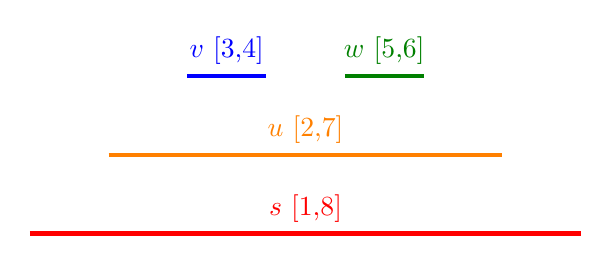
\begin{tikzpicture}
    \draw[ultra thick,red] (1,1) --node[above]{$s$ [1,8]} (8,1);
    \draw[ultra thick,orange] (2,2) --node[above]{$u$ [2,7]} (7,2);
    \draw[ultra thick,color=Green] (5,3) --node[above]{$w$ [5,6]} (6,3);
    \draw[ultra thick,blue] (3,3) --node[above]{$v$ [3,4]} (4,3);
  \end{tikzpicture}
\end{center}

Notice that the intervals shrink with depth and follow a structure
similar to the well-formed parenthesis problem.
We can in fact prove:

\begin{lemma}[parentheses theorem]\label{lem:dfs:paren}
  If $\vv{start}[u] < \vv{start}[v]$, then either $\vv{finish}[u] < \vv{start}[v]$
  or $\vv{finish}[u] < \vv{finish}[v]$.
\end{lemma}
\begin{prf}
  If $\vv{start}[u] < \vv{start}[v]$, we push $v$ on the stack
  while $u$ is still there, so we pop $v$ before we pop $u$ since stacks are FIFO.
\end{prf}

\section{Cut Vertices by DFS}
\lecture{(06/06)}

We define a cut vertex analogous to a bridge edge from MATH 239.

\begin{defn*}[cut vertex]
  Given a connected graph $G$,
  a vertex $v \in V(G)$ is a \term*{cut vertex} (or \term{articulation point})
  if removing $v$ and its edges makes $G$ disconnected.
\end{defn*}

\begin{example}
  \tikz\graph[empty nodes, nodes={circle, draw, fill, inner sep=2pt}]{
    1--{2,3[red]}-!-{4,5}--{6,7};
    2--3--{4,5}; 4--5--6--7;
  };
  has a cut vertex in \textcolor{red}{red}.
\end{example}

\begin{problem}
  Which of the vertices in $G$ are cut vertices?
\end{problem}

Consider a rooted DFS tree $T$ with known $\vv{parent}$ and $\vv{level}$.

\begin{prop}
  The root $s$ is a cut vertex if and only if it has more than one child.
\end{prop}
\begin{prf}
  Suppose $s$ has one child $v$.
  Then, $T-s$ is a rooted DFS tree with root $v$ (i.e., it remains connected).

  Suppose $s$ has subtrees $S_1,\dotsc,S_k$. 
  Let $u \in S_i$ and $v \in S_j$ for $i \neq j$.
  Then, there does not exist a path $u \leadsto v$ in $T - s$
  by the \nameref{lem:dfs:key-prop} since it would involve a non-tree, non-back cross edge.
  Therefore, the subtrees are disconnected in $T - s$.
\end{prf}

\begin{prop}
  Let $a(v) = \min\{\vv{level}[w] : vw \in E(G)\}$
  and $m(v) = \min\{a(w) : \text{$w$ descendant of $v$}\}$.
  Any non-root vertex $v$ is a cut vertex if and only if
  it has a child $w$ with $m(w) \geq \vv{level}[v]$.
\end{prop}
\begin{prf}
  Let $w$ be a child of $v$ with subtrees $T_w$ and $T_v$, respectively.

  Suppose $m(w) < \vv{level}[v]$ and we have removed $v$.
  Then, there is a vertex $w'$ in $T_w$ to some vertex $v'$ above $v$.
  That is, for any vertex $u \in V(T_w)$, we have that
  $u \leadsto w \leadsto w' \leadsto v' \leadsto s$
  and $T_w$ is still connected.

  Therefore, for $v$ to be a cut vertex, we must have $m(w) \geq \vv{level}[v]$.

  Suppose $m(w) \geq \vv{level}[v]$.
  Then, by the \nameref{lem:dfs:key-prop},
  all edges from $T_w$ end in $T_v$.
  They are either the tree edge $vw$
  or a back edge going to an ancestor at or below $v$.
  Therefore, removing $v$ will cause $T_w$ to be disconnected and $v$ is a cut vertex.
\end{prf}

Therefore, we can solve the cut vertex problem by calculating $m(v)$ for every vertex.

We can compute $a(v)$ in $O(\deg v)$.
Notice that if $v$ has children $w_1,\dotsc,w_k$,
then $m(v) = \min\{a(v), m(w_1), \dotsc, m(w_k)\}$.
Then, if we have the $m$ of the children, we get $m(v)$ in $O(\deg v)$.

By traversing the DFS tree, we get every $m(v)$ in $O(n+m) = O(m)$ (since $G$ connected).
Then, we can test the cut vertex condition for each vertex $v$
and each of its children in $O(\deg v)$.

Therefore, we can test all vertices in $O(m)$ time.

\begin{algorithm}[H]
  \caption{\Call{FindCutVertices}{$G$, $s$}}
  \begin{algorithmic}[1]
    \State $T \gets \Call{DFS}{G, s}$
    \Comment{DFS tree for $G$ with $\vv{root}$ and $\vv{level}$}
    \State $a, m \gets$ arrays of size $\abs{V(G)}$ initialized to $\infty$
    \State $\vv{cut} \gets$ array of size $\abs{V(G)}$ initialized to $\bot$
    \Procedure{Explore}{$v$}
    \For{$w$ child of $v$}
    \State $a[v] \gets \min\{a[v], \vv{level}[w]\}$
    \State \Call{Explore}{w}
    \State $m[v] \gets \min\{m[v], a[w]\}$
    \EndFor
    \State $m[v] \gets \min\{a[v], m[v]\}$
    \For{$w$ child of $v$}
    \If{$m[w] \geq T.\vv{level}[v]$} $\vv{cut}[v] \gets \top$ \EndIf
    \EndFor
    \EndProcedure
    \State \Call{Explore}{$T.\vv{root}$}
  \end{algorithmic}
\end{algorithm}

\section{Directed Graphs}

We can define a directed graph similar to an ordinary graph:

\begin{defn}[directed graph]
  A graph $G = (V, E)$ where edges are \emph{ordered} pairs $(u, v)$.
  If $G$ has no cycles, it is a \term{directed acyclic graph} (DAG).
\end{defn}

Note that we allow loops $(v, v)$.
Paths and cycles have the ordinary meaning.

\begin{defn}[topological ordering]
  An ordering $<$ of $V$ in a DAG such that $(a,b) \in E$ implies $a < b$.
\end{defn}

\lecture{(06/08)}
\begin{prop}
  A directed graph is acyclic if and only if there is a topological ordering on it.
\end{prop}
\begin{prf}
  The backwards direction is clear.

  Assume we have a DAG.
  There exists at least one vertex with in-degree 0,
  because otherwise there would be a cycle.
  We can inductively remove the vertex with in-degree 0 to get a topological ordering.

  In fact, if run DFS and we order $V$ with the ordering
  $v < w \iff \vv{finish}[w] < \vv{finish}[v]$,
  then we can show that $<$ is a topological order.

  Suppose that $(v, w) \in E$.
  
  If we discover $v$ before $w$, then $w$ is a descendant of $v$
  by the \nameref{lem:dfs:white-path} so we must finish exploring it before we finish $v$.

  Otherwise, if we discover $w$ before $v$,
  then there cannot exist a path $w \leadsto v$
  because otherwise $w \leadsto vw$ is a cycle.
  Therefore, $\vv{finish}[w] < \vv{start}[v] < \vv{finish}[v]$.

  Therefore, $<$ is a topological order whose existence
  is necessary and sufficient for a DAG.
\end{prf}

\begin{defn*}[strong connectivity]
  A directed graph $G$ is \term{strongly connected} if for all $v$ and $w$ in $G$,
  there is a path $v \leadsto w$ (and $w \leadsto v$)
\end{defn*}

\begin{corollary}
  $G$ is strongly connected if and only if there exists $s$
  such that for all $w$ there exist paths $s \leadsto w$ and $w \leadsto s$.
\end{corollary}
\begin{prf}
  The forwards direction is trivial.
  In the backwards direction, notice that for any two vertices $v$ and $w$,
  we have $v \leadsto s \leadsto w$ and $w \leadsto s \leadsto v$.
\end{prf}

\begin{problem}
  How can we test if a graph is strongly connected?
\end{problem}
\begin{sol}
  Call \Call{explore}{} twice, starting from the same vertex $s$.
  On the second run, reverse all the edges.
  Then, if every vertex $v$ is explored in both runs,
  we know that $s \leadsto v$ and $v \leadsto s$,
  i.e., the graph is strongly connected.

  We can reverse the edges using an adjacency list in $O(n+m)$ time,
  so this algorithm runs in $O(n+m)$ time.
\end{sol}

\begin{prop}
  Contracting the strongly connected components of a directed graph
  forms a DAG.
\end{prop}
\begin{prf}
  Suppose not. Then there exists a cycle of strongly connected components.
  However, this means that any vertex from any of these can be reached from any other.
  Therefore, the strongly connected component is not maximal.
\end{prf}

\lecture{(06/13)}
\begin{problem}
  What are the strongly connected components and their respective DAG?
\end{problem}
\begin{algorithm}
  \caption{Kosaraju's algorithm for strongly connected components}
  \begin{algorithmic}[1]
    \Procedure{SCC}{$G$}
    \State run \Call{DFS}{$G$} augmented with finish times
    \State sort the vertices by decreasing finish time
    \State run \Call{DFS}{$G\trans$}
    \State \Return{the trees in the DFS forest of $G\trans$}
    \EndProcedure
  \end{algorithmic}
\end{algorithm}

This has time complexity $O(n+m)$.

\begin{prop}
  For any vertices $v$ and $w$, \Tfae:
  $v$ and $w$ are in the same SCC; and
  $v$ and $w$ are in the same DFS tree of $G\trans$ (sorted by decreasing finish time).
\end{prop}
\begin{prf}
  Suppose $v, w \in C \in SCC(G)$ and let $s$ be the first vertex visited in $C$.
  Then, $s \leadsto v$ within $C$ and the path is white when visiting $s$ by supposition.
  By the \nameref{lem:dfs:white-path}, $v$ will be in the DFS tree.
  Likewise for $w$.

  Suppose $v$ and $w$ are in a DFS tree $T$ for $G\trans$ rooted at $s$.
  That is, among the vertices in $T$, $s$ has the highest finish time.
  Let $t \in T$.
  As a descendent, $s \leadsto_{G\trans} t$, so $t \leadsto_G s$.

  Claim that $t$ descends from $s$ in $G$, so we get a path $s \leadsto_G t$.

  Proceed by structural induction on $t$ and its children.
  Let $u$ be a child of $t$ in $T$.
  Suppose $\vv{start}[s] \leq \vv{start}[t] < \vv{finish}[t] \leq \vv{finish}[s]$.
  Since $\vv{finish}[u] < \vv{finish}[s]$, we have by the \nameref{lem:dfs:paren}
  that either $[s\ (u)]$ or $(u)\ [s]$.
  But the second option is impossible because if $tu \in E(T) \subseteq E(G\trans)$,
  then $ut \in E(G)$, which means that $u \leadsto t$ and by the \nameref{lem:dfs:white-path},
  $t$ should be a descendant of $u$, not $s$.
  Therefore, $u$ is a descendant of $s$, as desired.

  Finally, because $s \leadsto_G t$ and $t \leadsto_G s$,
  $t$ is in the strongly connected component of $s$.
\end{prf}

\begin{problem}
  Does a graph $G$ contain a Hamiltonian path (i.e., a path $P$ with $P(V) = V$)?
\end{problem}

For an undirected graph $G$, this is one of the canonical NP-complete problems.

For a DAG $G$, we can do this in linear time with a topological ordering.

\begin{prop}
  A DAG $G$ has a Hamiltonian path if and only if it has a topological ordering
  $v_1 < \dotsb < v_k$ such that $v_iv_{i+1} \in E(G)$ for all $i$.
\end{prop}
\begin{prf}
  Let $G$ have a Hamiltonian path $P = v_1\dotsb v_k$.
  Define an ordering $v_1 < \dotsb < v_k$.
  Suppose $v_i v_j \in E(G)$.
  If $i > j$, then $v_i v_j v_{j+1} \dotsb v_i$ is a cycle.
  However, $G$ is a DAG, so we must have $i < j$.
  Therefore, $<$ is a topological ordering as desired.

  Suppose $G$ has a topological ordering $v_1 < \dotsb < v_k$
  with $v_iv_{i+1} \in E(G)$ for all $i$.
  Then, we immediately get a Hamiltonian path given by $v_1 \dotsb v_k$.
\end{prf}
